\documentclass{beamer}

\usepackage{beamerthemeCambridgeUS}
\usepackage{graphics}
\usepackage{graphicx}
\usepackage{hyperref}
\usepackage{StyleFiles/algorithm}
\usepackage{StyleFiles/algorithmic}
\usepackage{amssymb}
\usepackage{fancyhdr}
\usepackage{eucal}
\usepackage[T1]{fontenc}
\usepackage{lmodern}
\usepackage{amsthm}

\title[Player Behavior and Team Strategy]{Player Behavior and Team Strategy in Robocup Simulation 3D League}
\author[Georgios Methenitis]{Georgios Methenitis}
\institute[TUC]{Technical University of Crete}
\date[Chania, 2012]{Chania, August, 2012}
\subject{Computational Sciences}

\begin{document}

\newcommand{\putat}[3]{\begin{picture}(0,0)(0,0)\put(#1,#2){#3}\end{picture}}

  \frame
  {
    \titlepage
    \begin{center}
    \begin{small}
     Thesis Committee\\
    Assistant Professor Michail G. Lagoudakis (ECE)\\
Assistant Professor Georgios Chalkiadakis (ECE)\\
Professor Minos Garofalakis (ECE)\\
    \end{small}
    \end{center}
  }

  
  \frame
  {
    \frametitle{Abstract}
    In this thesis we present...

  }  
  
  
  
  \section{Outline}

  \frame
  {
    \frametitle{Outline of Topics}

    \tableofcontents
  }

  \section{Background}

 \subsection*{RoboCup}
  \frame
  {
    \frametitle{Robocup Competition}
    RoboCup is an international robotics competition founded in 1997. The official goal of the project is stated as an ambitious endeavor: ``By the year 2050, a team of fully autonomous humanoid robot soccer players shall win the soccer game, complying with the official rule of the FIFA, against the winner of the most recent World Cup''.

  }
  
  \frame
  {
    \frametitle{Robocup Leagues}
   	\begin{description}
   	\item[Soccer] Popular, well-known Rules, cooperative multi-agent systems in dynamic adversarial environments.
   	\item[Rescue] Prompt support for planning disaster mitigation, search and rescue.
   	\item[@Home] Aims to develop service and assistive robot technology with high relevance for future personal domestic applications.
   	\item[Junior] It is designed to introduce RoboCup to primary and secondary school children
   	\end{description}

  }


  \subsection*{RoboCup Simulation Soccer}
  \frame
  {
    \frametitle{Soccer Simulation League}
    One of the oldest leagues in RoboCup's Soccer. The Simulation League focus on artificial 				intelligence and team strategy. Independently moving software players (agents) play soccer on a 	virtual field inside a computer. There are two sub-leagues: 2D and 3D.
    

  }
  
  \frame
  {
    \frametitle{2D vs 3D}
    \begin{figure}[t!] 
\centering
    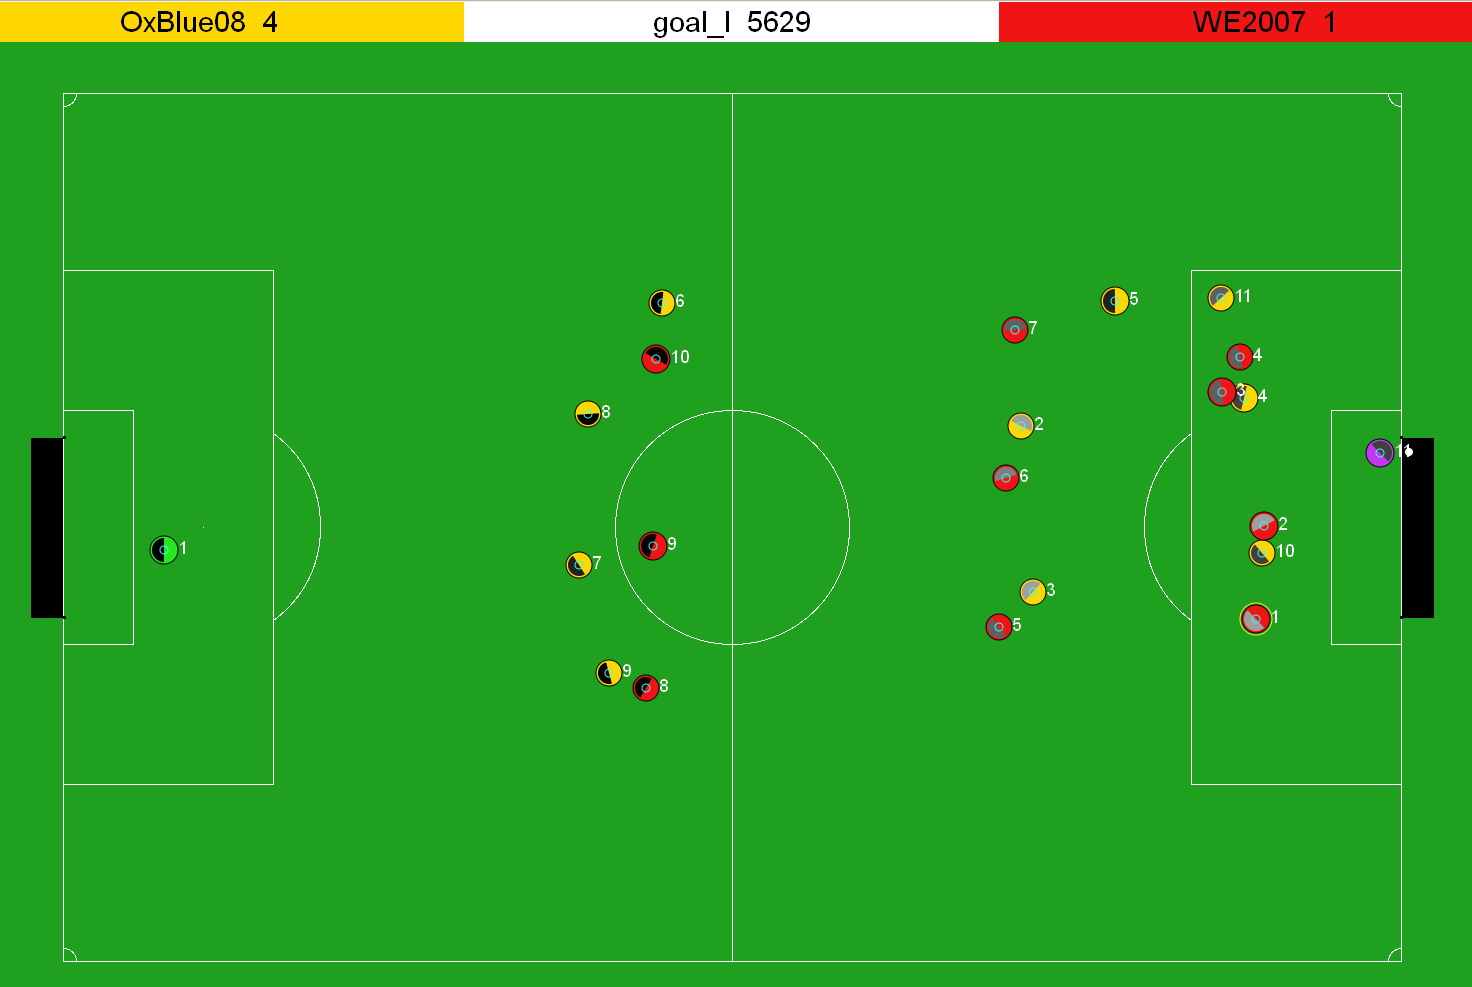
\includegraphics[height=3.5cm]{figures/2D.jpg}\	
    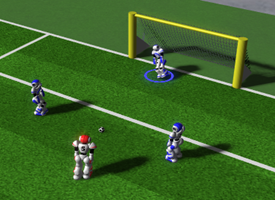
\includegraphics[height=3.5cm]{figures/3d.png}
\end{figure}
    

  }
  
  \subsection*{RoboCup 3D Simulation Soccer}
  \frame
  {
    \frametitle{3D Simulation Soccer}
    \begin{itemize}
    \item At its beginning, the only available robot model was a spherical agent.
    \item In 2006, a simple model of the Fujitsu HOAP-2 robot was made available, being the first time that humanoid models were used in the simulation league.
    \item In 2008, the introduction of a Nao robot model to the simulation gave another perspective to the league. 
    
    \item \textbf{SimSpark} is used as the official Robocup
3D simulator.
    \end{itemize}
         
  }
  
  \frame
  {
    \frametitle{SimSpark}
    \begin{itemize}
    \item \textbf{SimSpark} is a generic physics simulator system for multiple agents in three-dimensional
	environments.

	\item \textit{Rcssserver3d} is the official competition environment for the RoboCup 3D Simulation League. It implements a simulated soccer environment, whereby two teams of up to
	nine, and in the latest version up to eleven, humanoid robots play against each other.

    \end{itemize}
         
  }
  
  \frame
  {
    \frametitle{Server's Versions}
    \begin{itemize}
    \item Version 0.6.5
    \begin{description}
    \item[Players] 9
    \item[Length] 21m
    \item[Width] 14m
    \end{description}
    
    \item Version 0.6.6
     \begin{description}
    \item[Players] 11
    \item[Length] 30m
    \item[Width] 20m
    \end{description}
    \end{itemize}
         
  }
  
  \frame
  {
    \frametitle{Soccer Field}
    \begin{figure}[t!]
\centering
  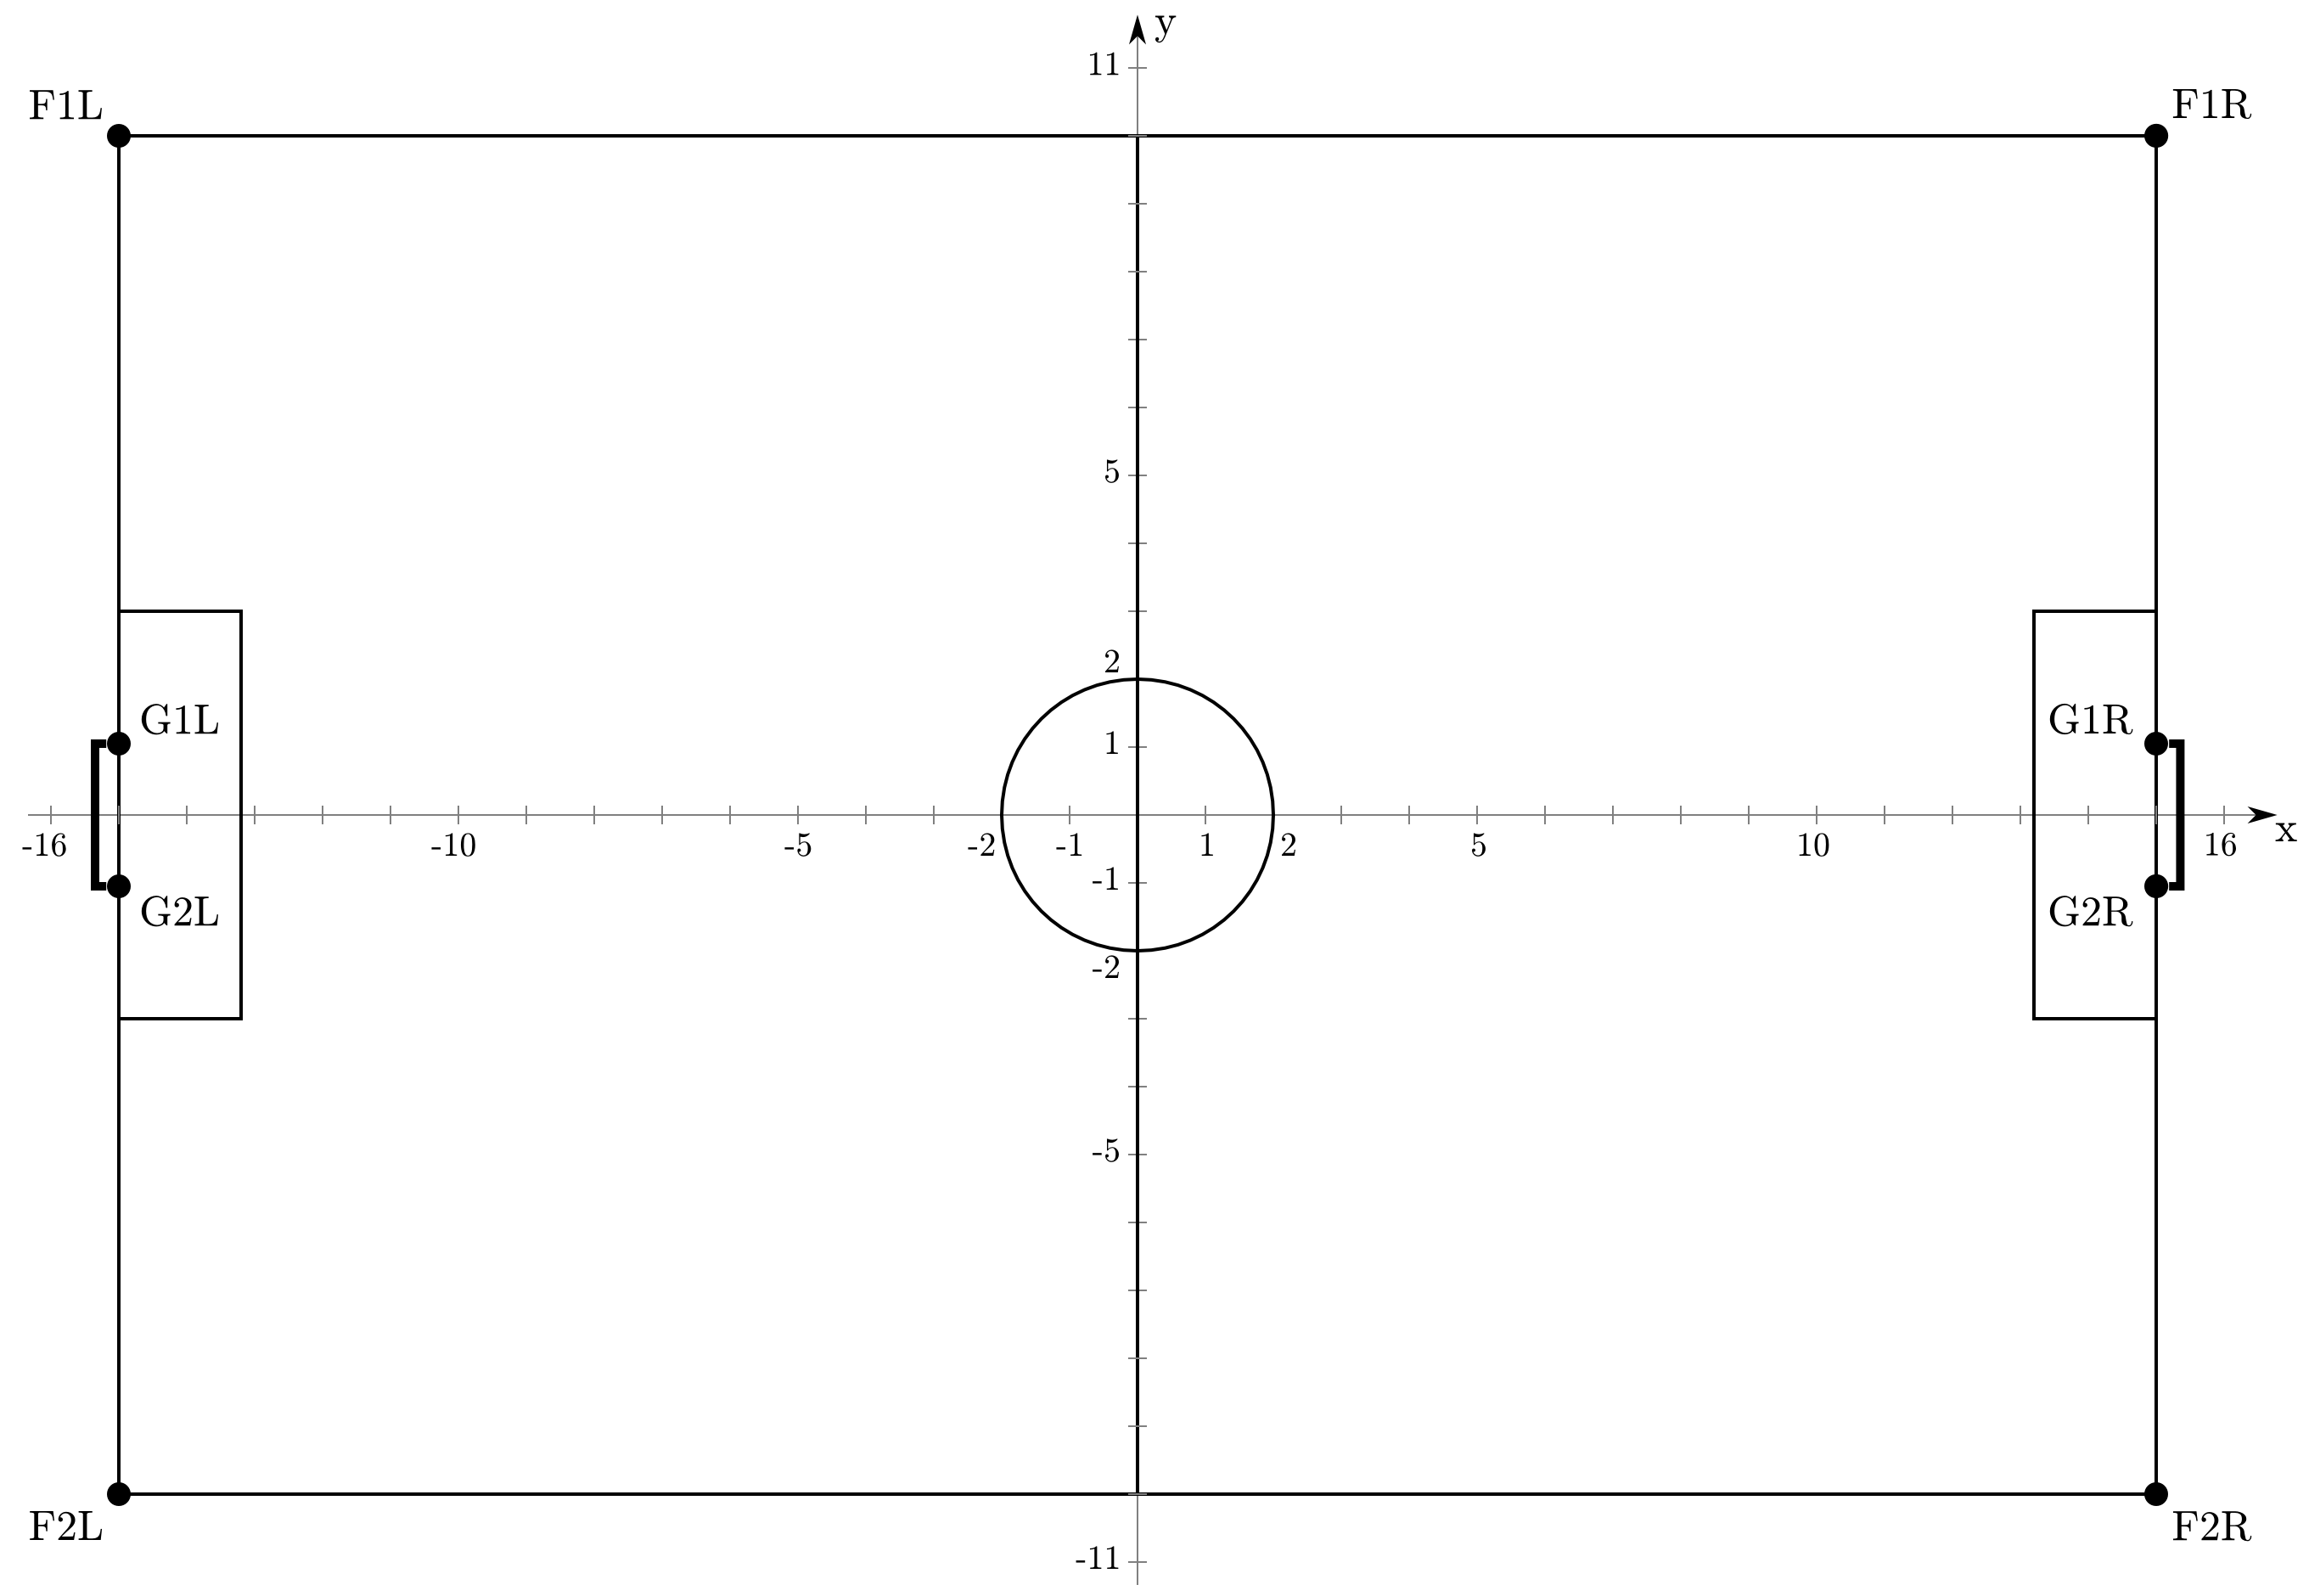
\includegraphics[width=0.8\textwidth]{figures/SoccerSimulation_FieldPlan.png}
\end{figure}
         
  }
  
  \frame
  {
    \frametitle{Robot Model}
    The Nao humanoid robot manufactured by Aldebaran Robotics. Its height is about 57cm and its 			weight is around 4.5kg. The simulated model comes with 22 degrees of freedom.
    \begin{figure}
\centering
  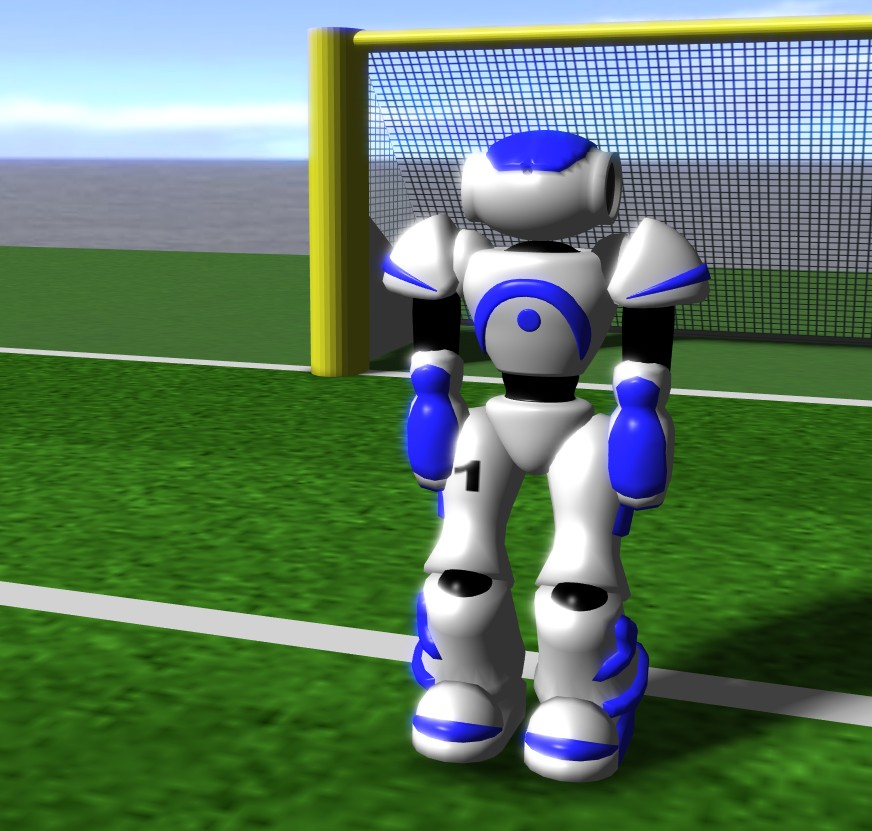
\includegraphics[trim=7cm 0cm 0cm 0cm, clip, width=0.4\textwidth]{figures/629px-Models-nao.jpg}
  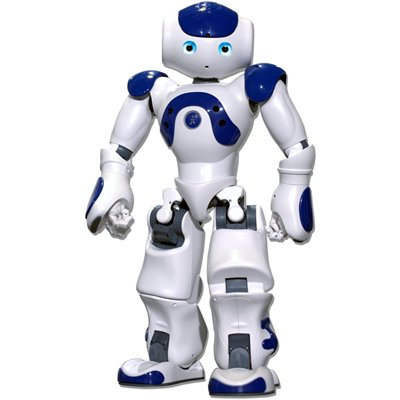
\includegraphics[width=0.4\textwidth]{figures/RealNao.jpg}
\end{figure}

   
  }
  
  \frame
  {
    \frametitle{Server}
    The SimSpark server hosts the process that manages and advances the simulation. The
	simulation state is constantly modified through the simulation update loop. Each simulation 			step corresponds to 20ms of simulated time.
	\begin{figure}[t!]
	\centering
  		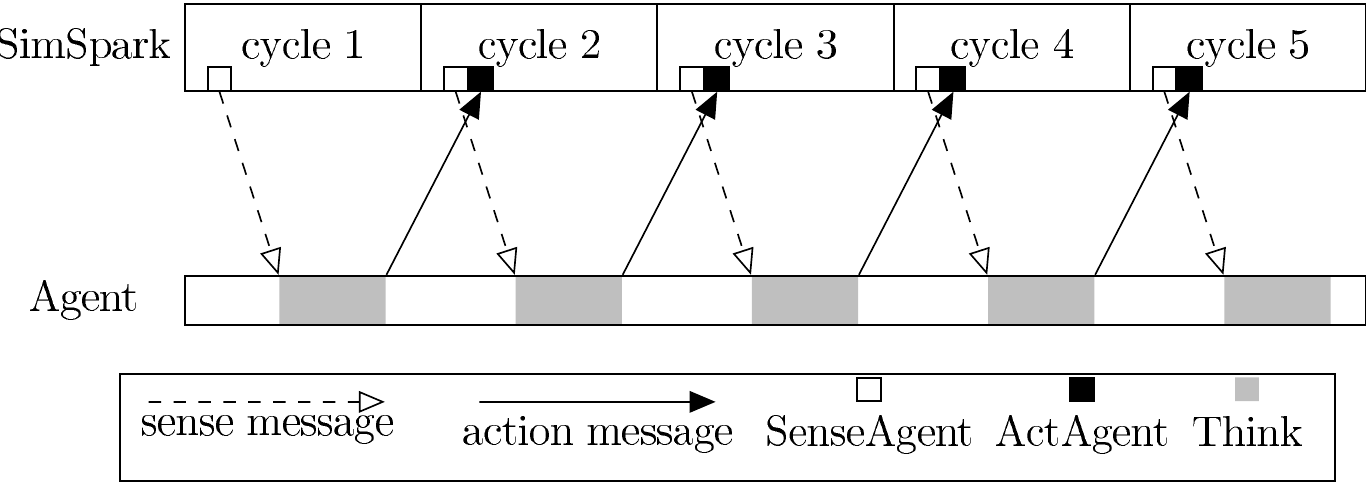
\includegraphics[width=0.6\textwidth]														{figures/SimulationUpdateLoopSynchronizationBetweenSimSparkAndAgent.png}
	\end{figure}
     
  }
  
  
  
  \frame
  {
    \frametitle{Monitor}
    \begin{itemize}
    \item SimSpark Monitor
    \begin{itemize}
    \item Responsible for rendering the current simulation
    \item Default SimSpark monitor
	\end{itemize}    

    \item RoboViz Monitor 
	\begin{itemize}
    \item Designed to assess and debug agent behaviors in the RoboCup 3D
Simulation League
    \item Allow drawing
    \item Official monitor of the RoboCup 3D simulation Soccer League
	\end{itemize}     
    \end{itemize}
    
     
  }
  
  \frame
  {
    \frametitle{Monitors Comparison}
    \begin{figure} 
  \begin{center}
    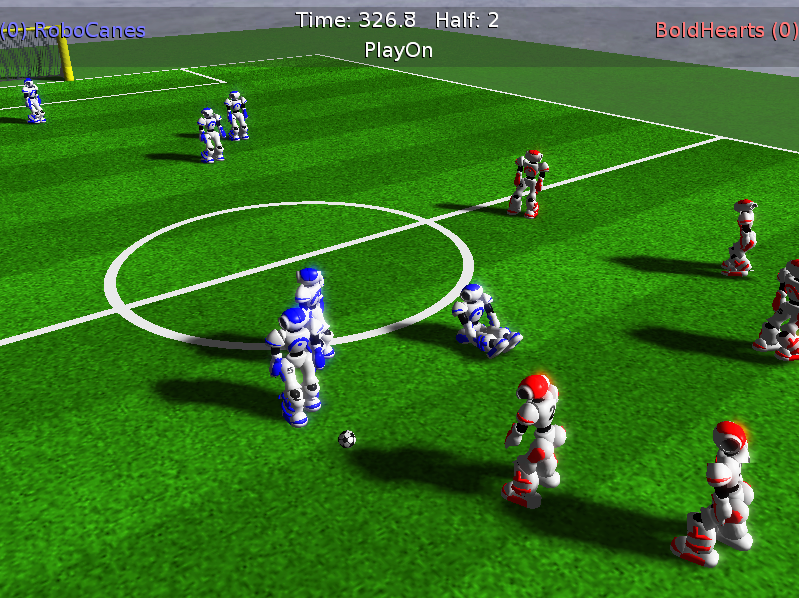
\includegraphics[width=0.45\textwidth]{figures/RobovizMonitor.png}\	
    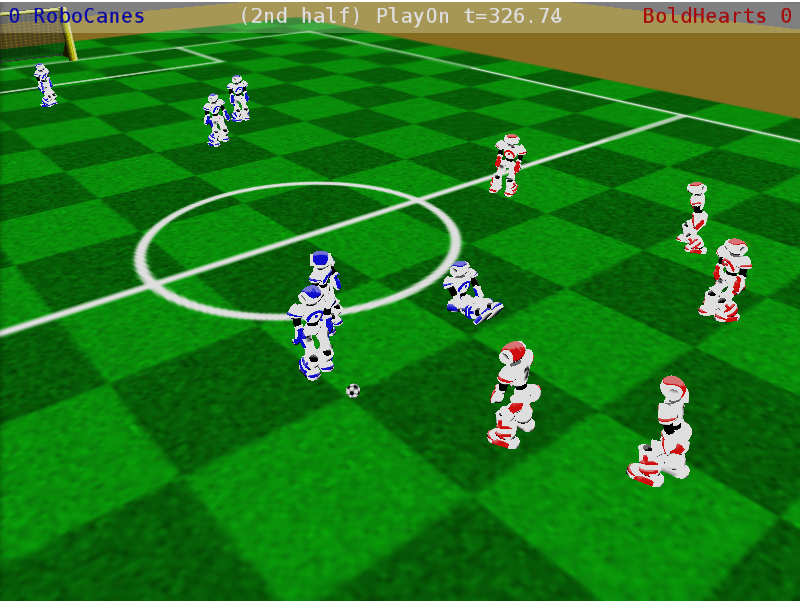
\includegraphics[width=0.45\textwidth]{figures/SimSparkMonitor.png}
  \end{center}
\end{figure}
    
     
  }
  

  \begin{frame}[allowframebreaks]
  \frametitle{Agent Perceptors}
Perceptors are the senses of an agent, allowing awareness of the agent's model state and the environment.  
  
    \begin{description}
    \item[HingeJoint Perceptor] A hinge joint perceptor receives information about the angle of
the corresponding single-axis hinge joint.
\begin{description}
  \item[{\bf Message format:}]
  \texttt{(HJ (n <name>) (ax <ax>))}
  \item[{\bf Frequency:}]
  Every cycle
  \end{description}

    \item[ForceResistance Perceptor] This perceptor informs about the force that acts on a
body.
\begin{description}
  \item[{\bf Message format:}]
  \texttt{(FRP (n <name>) (c <px> <py> <pz>) (f <fx> <fy> <fz>))}
  \item[{\bf Frequency:}]Only in cycles where a body collision occurs
  \end{description}

    \item[GyroRate Perceptor] The gyro-rate perceptor delivers information about the change
in orientation of a body.
\begin{description}
  \item[{\bf Message format:}]
  \texttt{(GYR (n <name>) (rt <x> <y> <z>))}
  \item[{\bf Frequency:}]
  Every cycle
  \end{description}

    \item[Accelerometer Perceptor] This perceptor measures the proper acceleration a body ex-
periences relative to free fall.
\begin{description}
  \item[{\bf Message format:}]
  \texttt{(ACC (n <name>) (a <x> <y> <z>))}
  \item[{\bf Frequency:}]
  Every cycle
  \end{description}

    \item[Vision Perceptor] Vision perceptor delivers information about seen objects in the environment, where objects are either others players, the ball, field lines, or markers on the field.
   \begin{description}
  \item[{\bf Message format:}]
  \texttt{(See +(<name> (pol <d> <a1> <a2>))}\\
  \texttt{+(P (team <name>) (id <ID>) +(<bodypart> (pol <d> <a1> <a2>)))}\\
  \texttt{+(L (pol <d> <a1> <a2>)(pol <d> <a1> <a2>)) )}\\
  \item[{\bf Frequency:}]
 Every third cycle (60ms)
  \end{description}

    \item[Hear Perceptor] Hear perceptor serves as an
aural sensor and receives messages shouted by other players.
\begin{description}
  \item[{\bf Message format:}]
  \texttt{(hear <time> self/<direction> <message>)}
  \item[{\bf Frequency:}]
  Only in cycles, where a message is heard
  \end{description}

    \item[GameState Perceptor] The game state perceptor delivers information about the ac-
tual state of the soccer game environment.
\begin{description}
  \item[{\bf Message format:}]
  \texttt{(GS (t <time>) (pm <playmode>))}
  \item[{\bf Frequency:}]
 Every cycle
  \end{description}

    \end{description}
  \end{frame}
  
  \begin{frame}[allowframebreaks]
    
    \frametitle{Agent Effectors}
    Effectors allow agents to perform actions within the simulation. Agents control them by sending messages to the server and the server changes the game state accordingly.
    
    
    
    \begin{description}
    
    
    \item[Create Effector]An agent uses this effector to advice the server to construct the physical representation and all further effectors and perceptors of the agent in the simulation environment according to a scene description file it passes as a parameter.
    
    
    \begin{description}
  \item[{\bf Message format:}]
  \texttt{(scene <filename>)}
  \item[{\bf Frequency:}]
  Only once
  \end{description}
  
  
    \item[HingeJoint Effector] Effector for all axes with a single degree of freedom.
    
    
    \begin{description}
  \item[{\bf Message format:}]
  \texttt{(<name> <ax>)}
  \item[{\bf Frequency:}]
  Once per cycle maximum
  \end{description}
  
  
    \item[Synchronize Effector]Agents running in Agent Sync Mode must send this command at the end of each simulation cycle.
    
    
    \begin{description}
  \item[{\bf Message format:}]
  \texttt{(syn)}
  \item[{\bf Frequency:}]
  Every cycle
  \end{description}
  
  
    \item[Init Effector]The init effector registers the agent as a member of a team with a specific player number.
    
    
    \begin{description}
  \item[{\bf Message format:}]  
  \texttt{(init (unum <playernumber>) (teamname <teamname>) )}
  \item[{\bf Frequency:}]
  Only once
  \end{description}
  
  
    \item[Beam Effector]The beam effector allows a player to position itself anywhere on the field only before any kick-off.
    
    
    
    \begin{description}
  \item[{\bf Message format:}]  
  \texttt{(beam <x> <y> <rot>)}
  \item[{\bf Frequency:}]
  Once before each kick-off
  \end{description}
  
  
  
    \item[Say Effector]The say effector permits communication among agents by broadcasting messages in plain ASCII text (20 characters maximum).
    
    
    
    \begin{description}
  \item[{\bf Message format:}]
  \texttt{(say <message>)}
  \item[{\bf Frequency:}]
  Once per cycle maximum
  \end{description}
    \end{description}
       
     
  \end{frame}
  


  \section{Player Skills}

 \subsection*{General Skills}

  \frame
  {
    \frametitle{Architecture}
    \begin{itemize}
    \item Connection with Server
    \item Update Beliefs and Sensors' Data
    \item Localization Process
    \item Locomotion
    \item Actions
    \item Agent Behavior
    \item Communication
    \item Team Coordination
    \end{itemize}
    

    
  }





 \frame
  {
    \frametitle{Architecture}
    
    \begin{figure}
	\centering
 	 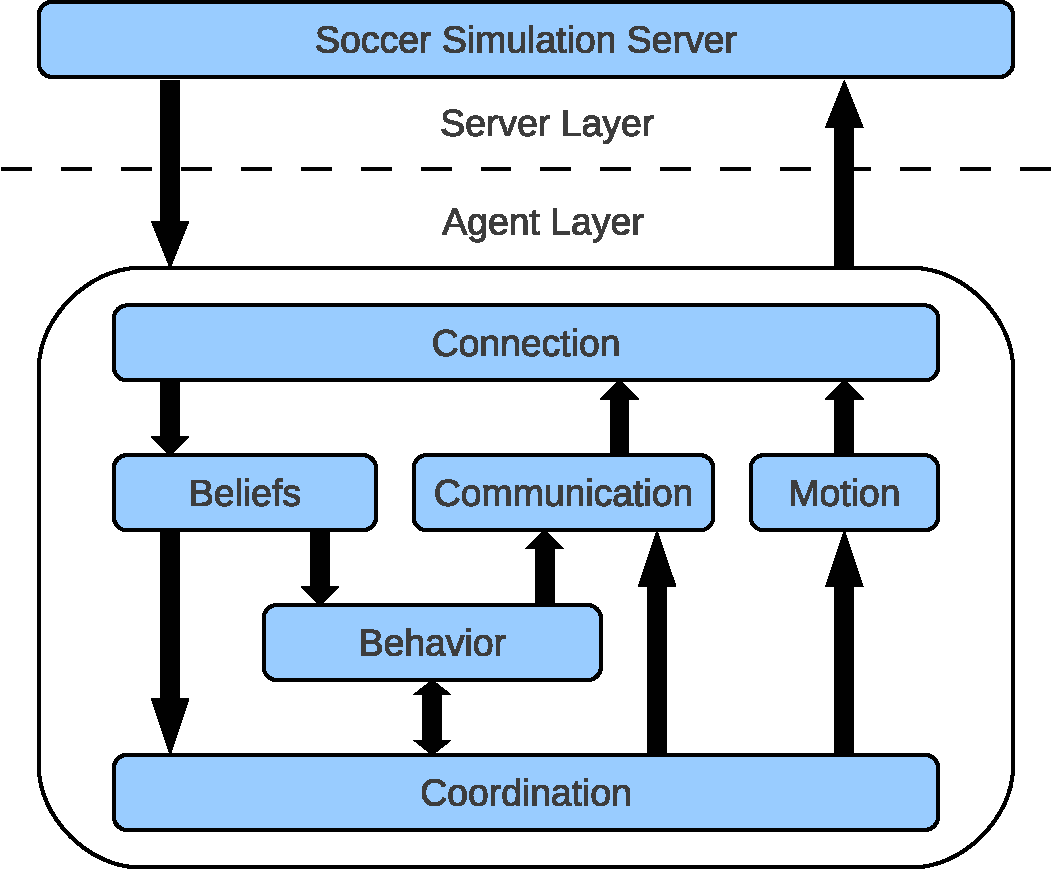
\includegraphics[width=0.7\textwidth]{figures/Arch.pdf}
	\end{figure}

    
  }


  \frame
  {
    \frametitle{Connection}
    
	\begin{itemize}
    \item Agent has to be connected to the server at all times during a simulated game.
    \pause
    \item Agent
receives sense messages from the server every 20ms at the beginning of each simulation
cycle.

    \pause
    \item Agents willing
to send action messages, can do so at the end of their think cycles, which may or may not
coincide with the simulation cycles.

    \end{itemize}

    
  }
  
  \frame
  {
    \frametitle{Perception}
    \begin{itemize}
	 \item Perceptions in simulated soccer are quite different compared to those in real soccer 			games.
    \pause
    \item Agents do not have to process raw data coming directly from sensors, but rather listen
	to sensor and higher-level observation messages sent by the server at each cycle.
	\pause
    \item Agents update their beliefs and store sensors' data parsing these messages.
 	\end{itemize}


    
  }
  
  \begin{frame}[fragile]
  \frametitle{Sense Message Example}
  \begin{footnotesize}
  \begin{verbatim}(time (now 46.20))(GS (t 0.00) (pm BeforeKickOff))(GYR (n torso)
(rt 0.00 0.00 0.00))(ACC (n torso) (a 0.00 -0.00 9.81))(HJ (n hj
1)(ax 0.00))(HJ (n hj2) (ax 0.01))(See (G2R (pol 14.83 -11.81 1.
08))(G1R (pol 14.54 -3.66 1.12)) (F1R (pol 15.36 19.12 -1.91))(F
2R (pol 17.07 -31.86 -1.83)) (B (pol 4.51 -26.40 -6.15)) (P (tea
m AST_3D)(id 8)(rlowerarm (pol 0.18 -35.78 -21.65)) (llowerarm (
pol 0.19 34.94-21.49)))(L (pol 8.01 -60.03 -3.87) (pol 6.42 51.1
90 -39.13 -5.17))(L (pol 5.91 -39.06 -5.11) (pol 6.28-29.26 -4.8
8)) (L (pol 6.28 29.34 -4.95)(pol 6.16 -19.05 -5.00)))(HJ(n raj1
) (ax -0.01))(HJ (n raj2) (ax -0.00))(HJ (n raj3)(ax -0.00))(HJ(
n raj4) (ax 0.00))(HJ (n laj1) (ax 0.01))(HJ (n laj2) (ax 0.00)) ...
  \end{verbatim}
  \end{footnotesize}
\end{frame}


  \subsection*{Localization}
  \frame
  {
    \frametitle{Self-Localization}
    
	\begin{itemize}
	\item Localization is executed every three cycles (60ms).
    \pause
    \item Localization uses the eight visible landmarks into the field.
    \begin{itemize}
    \item G1R, G2R
    \item G1L, G2L
    \item F1R, F2R
    \item F1L, F2L
    \end{itemize}
	\pause
    \item A key restrictive factor is that the agents are equipped with a restricted vision 				perceptor which limits the field of their view to 120 degrees.

 	\end{itemize}

  }
  

  \frame
  {
    \frametitle{Simulated Nao's Field of View}

   \begin{figure}
	\centering
  	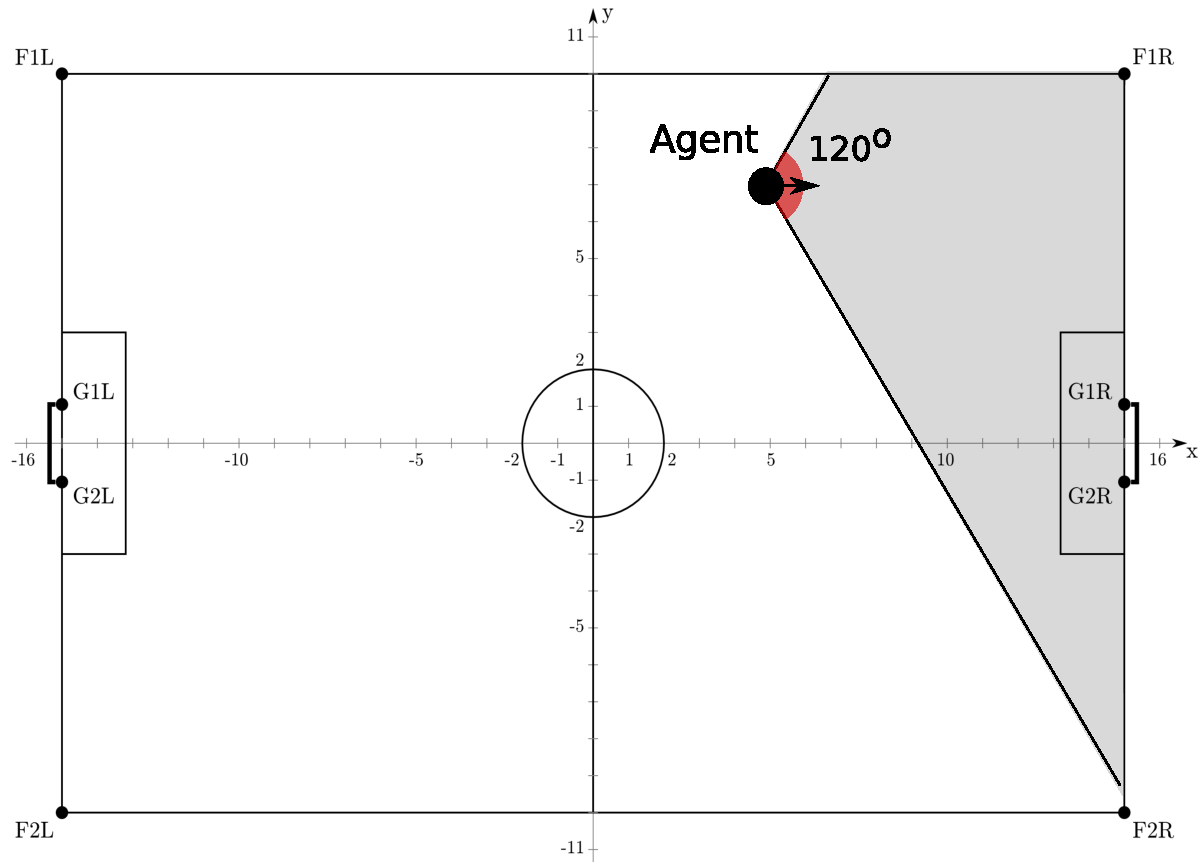
\includegraphics[width=0.8\textwidth]{figures/LViewAngle.pdf} 		
	\end{figure}
    
  }
    
  
  \frame
  {
    \frametitle{Self-Localization Technique}
	\begin{figure}
	\centering
  	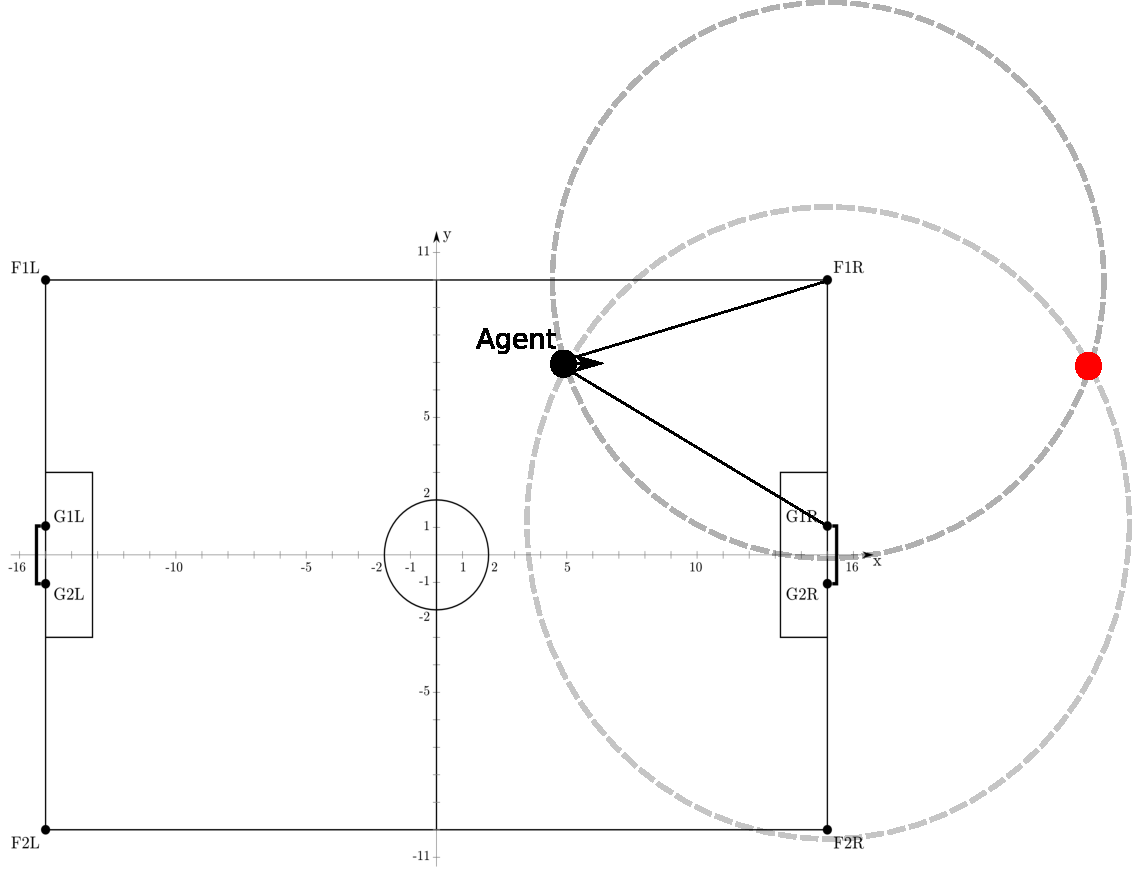
\includegraphics[width=0.8\textwidth]{figures/Localization.pdf}
	\end{figure}
   
    
  }
  
  \frame
  {
    \frametitle{Object Localization}
	\begin{itemize}
	\item Computing the position of other visible objects.
	\pause
	\begin{itemize}
	\item Other Players
	\item Ball
	\end{itemize}
	\pause
    \item Information about Visible Objects
    \pause
    \begin{itemize}
	\item Distance
	\item Horizontal, Vertical Angles
	\end{itemize}
	\pause
	\item Enough information to compute those objects' positions if we know our exact position.
 	\end{itemize}
   
    
  }
  
  \frame
  {
    \frametitle{Localization Filtering}
	\begin{itemize}
	\item Absence of a more sophisticated probabilistic localization scheme.
	\pause
	\item Temporary absences of landmarks.
	\pause
	\item Noisy observations.
	\end{itemize}
   
    
  }
 
  \frame
  {
    \frametitle{Localization Filtering Algorithm}
\begin{algorithm}[H]
\caption{Localization Filtering}
\label{LocalizationFiltering}
\begin{algorithmic}[1]
\begin{footnotesize}
\STATE {\bf Input: }$LastEstimate$
\STATE {\bf Output: }$FilteredLocation$
\STATE $Queue$: a FIFO queue storing the $MaxSize$ (default=10) most recent estimates
\STATE 
\IF{$size(Queue) = 0$}
\STATE $Queue.Add(LastEstimate)$
\ELSIF{$LastEstimate \not\approx AverageLocation(Queue)$}
\STATE $Queue.Remove()$
\ELSE 
\IF{$size(Queue) = MaxSize$}
\STATE $Queue.Remove()$
\ENDIF
\STATE $Queue.Add(LastEstimate)$
\ENDIF
\RETURN $AverageLocation(Queue)$
\end{footnotesize}
\end{algorithmic}
\end{algorithm}
   
    
  }
  
  
  \subsection*{Motions and Movement}
  
  
  \frame
  {
    \frametitle{Nao's Anatomy}
    The simulated Nao robot comes with 22 degrees of freedom, corresponding to 22 hinge
joints. Figure 4.6 shows Nao�s anatomy with all joints, split in five kinematic chains
(head, left arm, right arm, left leg, right leg).
\begin{figure}
\centering
  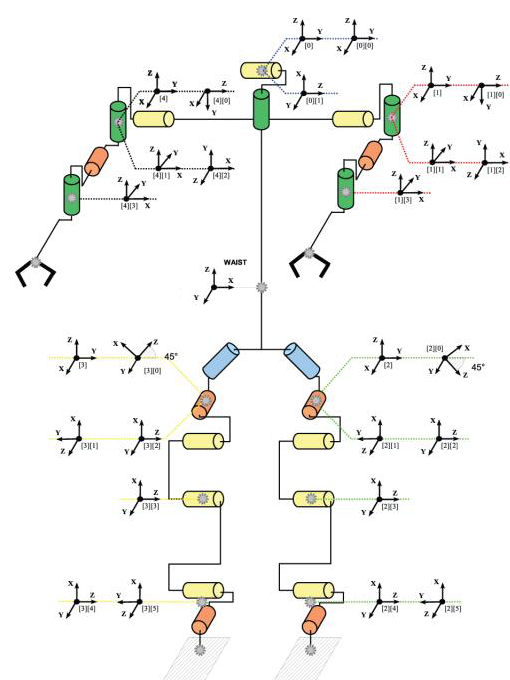
\includegraphics[width=0.3\textwidth]{figures/Models_NaoAnatomy.png}
\end{figure}

  }
  
  \frame
  {
    \frametitle{Motion and Movement}
    In robotics, a complex motion is commonly defined as a sequence of timed joint poses. A pose is a set of values for every joint in the robot's body or in a specific kinematic chain at a given time. 
For any given set of $n$ joints a pose at time $t$ is defined as:
\[
Pose(t)= \lbrace J_{1}(t), J_{2}(t), \ldots ,J_{n}(t) \rbrace
\]

  }
  
  \begin{frame}[fragile]
  \frametitle{XML-Based Motion Files}
  \begin{tiny}
  \begin{verbatim}<phase name="Start" next="Phase1">
   <effectors>
      Joint Values
   </effectors>
   <duration>duration</duration>
</phase>

<phase name="Phase1" next="Phase2">
   <effectors>
      Joint Values
   </effectors>
   <duration>duration</duration>
</phase>

<phase name="Phase2" next="Phase1">
   <effectors>
      Joint Values
   </effectors>
   <duration>duration</duration>
   <finalize>Final</finalize>
</phase>

<phase name="Final">
   <effectors>
      Joint Values
   </effectors>
   <duration>duration</duration>
</phase>
  \end{verbatim}
  \end{tiny}
  
  \putat{200}{30}{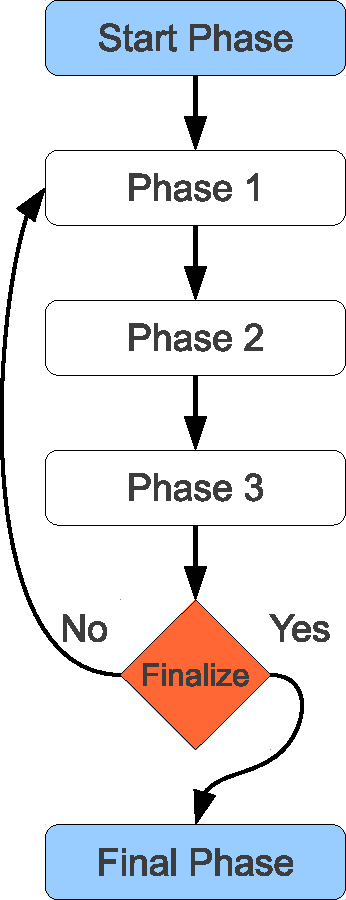
\includegraphics[width=0.2\textwidth]{figures/MotionSequence.pdf}}
  
\end{frame}


\frame
  {
    \frametitle{XML-Based Motion Controller}
    To generate motions for our agent we need to create a motion string, which encloses information about each joint's velocity. This velocity is computed as follows:
\[
Joint Velocity = \cfrac{Desired Joint Value - Current Joint Value}{PhaseDuration}
\]
A velocity value is calculated for each joint involved in the motion and the final output of the motion controller is sent to the server. In addition, zero velocity is set for every joint not included in the \texttt{effector} field of each phase, so that they stop moving. 

  }
  
  
   
 \begin{frame}[fragile]
  \frametitle{Text-Based Motion Files}
  \begin{footnotesize}
  \begin{verbatim}#WEBOTS_MOTION,V1.0
LHipYawPitch,LHipRoll,LHipPitch,LKneePitch,LAnklePitch,...
00:00:000,Pose1,0,-0.012,-0.525,1.05,-0.525,0.012,0,...
00:00:040,Pose2,0,-0.011,-0.525,1.05,-0.525,0.011,0,...
00:00:080,Pose3,0,-0.009,-0.525,1.05,-0.525,0.009,0,...
00:00:120,Pose4,0,-0.007,-0.525,1.05,-0.525,0.007,0,...
00:00:160,Pose5,0,-0.004,-0.525,1.05,-0.525,0.004,0,...
00:00:200,Pose6,0,0.001,-0.525,1.051,-0.525,-0.001,0,...
00:00:240,Pose7,0,0.006,-0.525,1.05,-0.525,-0.006,0,...
00:00:280,Pose8,0,0.012,-0.525,1.05,-0.525,-0.012,0,...
00:00:320,Pose9,0,0.024,-0.525,1.05,-0.525,-0.024,0,...
\end{verbatim}
  \end{footnotesize}
\end{frame}

\frame
  {
    \frametitle{Text-Based Motion Controller}
    The motion controller could be customized easily to perform these motions in different ways. The following parameters can be modified:
\begin{description}
	\item[Duration] The time between poses in simulation cycles. By default, $Duration=2$.
	\item[PoseStep] The step for advancing from pose to pose. By default, $PoseStep=1$, but we can subsample the motion with other values, e.g. for $PoseStep=2$, we execute pose1, pose3, pose5, ...
\end{description}
The desired velocity of each joint is computed by:
\[
JointVelocity = \cfrac {Desired Joint Value - Current Joint Value} {Duration \times CycleDuration}
\]
A velocity value is calculated for each joint involved in the motion and the final output of the motion controller is sent to the server. 

  }
  
  
\frame
  {
    \frametitle{Dynamic Motion Elements}
    \begin{description}
    \item[Walk Leaning] The XML-based walk motion can be dynamically modified to lean to
the right or to the left. This is accomplished by altering the joint values of the (left
or right) HipPitch and AnkePitch joints in specific phases of the walk motion.

    \item[Walk Slowdown] Increasing the phase durations dynamically by about 35\% yields a smooth approach to a stopping position.

    \item[Dynamic Turn] The text-based turn motion can be dynamically modified using a gain value
for scaling the resulting velocities in order to perform the motion in a smoother or
rougher way. By dynamically changing this value between 0.3 and 1.0, the agent is able to turn its body anywhere between 3 and 40 degrees.

    \end{description}

  }
  
  \frame
  {
	\begin{description}
	\item[X-Axis] Gain factor
	\item[Y-Axis] Agent turn
\end{description}	    
    
    \frametitle{Dynamic Turn Example}
    \begin{figure}
	\centering
 	 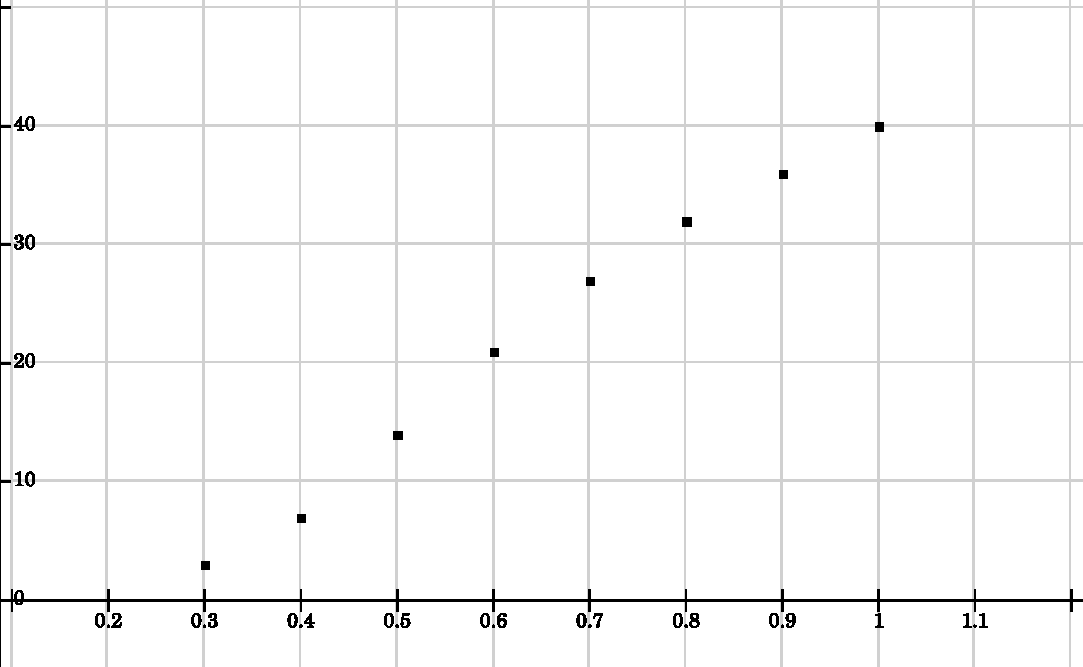
\includegraphics[width=0.8\textwidth]{figures/DynamicTurn.pdf}
	\end{figure}
  }
  
  
  \subsection*{Actions}
  \begin{frame}

    \frametitle{Actions}
    Actions are split into groups in terms of their complexity:
    \begin{description}
    \item[Basic Actions] Basic actions combine perceptual information and motion files in simple ways to achieve something useful.
    \item[Complex Actions] Complex actions combine perceptual information, motion files, and basic actions. They have a more complicated structure and aim to achieve specific goals.
    \end{description}
  
  \end{frame}
  
  \begin{frame}[allowframebreaks]
    \frametitle{Simple Actions}
	\begin{description}
    \item[Look Straight] Straight Moves the head to its nominal position. Both head joints are set to $0$.
    \item[Scan] Moves the head to perform periodic panning and tilting. 
    \item[Pan Head] Moves the head to perform periodic panning at zero tilt.
    \item[Track Object] Moves the head to bring a particular object to the center of the field of view. This action is applicable only when the object being tracked is visible, but is limited by the joint ranges. 
    \item[Track Moving Object] This action estimates the direction and the speed of a moving object using a small number of observations, obtained while performing the Track Object action. It records a set of five consecutive observations and another set of five consecutive observations delayed by a fixed time period (the default is 5 cycles).  The difference between the average positions of each set gives a vector that reveals the direction of motion. Taking the ratio of the magnitude of this vector and the time delay yields the speed of the moving object.
    \item[Find Opponent�s Goals] This action estimates the direction of the opponent's goal with respect to the agent by performing the Scan action.
	\item[Look For Ball] Turns the body of the agent, while performing the Scan action, until the ball appears within the field of view.
	\item[Turn To Ball] Turns the body of the agent towards the direction of the ball, while performing the Track Ball action. It can applied only when a ball is visible.
	\item[Turn To Localize] Turns the body of the agent, while performing the Pan Head action, until the agent's belief about its own location is updated with confidence.
	\item[Stand Up] Makes the agent stand up on its feet, after a confirmed fall on the ground, whether face-up or face-down. This action monitors the inertial sensors (accelerometers and gyroscopes) to check if our agent has fallen on the ground. Incoming gyroscope and accelerometer values above a specific threshold indicate a possible fall, but this has to be confirmed, because it is not unusual to receive values above threshold due to collisions without a fall. To confirm a fall, the action checks the force resistance perceptors located under the agent's feet. If these perceptors imply that the legs do not touch the ground, then we are pretty sure that a fall has occurred. In this case, a stand up motion is executed. Foot pressure values are also used to determine whether the stand up motion succeeded or not. The stand up motion is repeated, until it succeeds. 
	\item[Prepare for Kick] Positions the agent to an appropriate position with respect to the ball in order to perform a kick successfully.
    \end{description}

  \end{frame}
  
  \begin{frame}[allowframebreaks]
    \frametitle{Complex Actions}
    \begin{description}
    \item[Avoid Obstacles]
	\begin{itemize}
	\item Simulated Nao's head can pan from $-120^{\circ}$ to $+120^{\circ}$ and the field of view is $120^{\circ}$, we can obtain a complete imaging of all obstacles located close to our agent.
	\item For each recorded obstacle, we calculate two escape angles that determine the two directions which guarantee avoidance of the obstacle at a safe distance.
	\item Any escape angle of some obstacle that falls within the forbidden area of some other obstacle is discarded.
	\item Any escape angle of some obstacle that falls within the forbidden area of some other obstacle is discarded.
	\item The remaining escape angles, and particularly the escape way points they define (the points closest to the obstacle along the direction of the escape angles), are evaluated in terms of the angle and distance overhead they incur with respect to the agent orientation (for the angle) and the target (for the distance).
	\item The way point that minimizes the total overhead is selected as a temporary target for avoiding the obstacles, while making progress towards the target.
	

\begin{figure}
\centering
  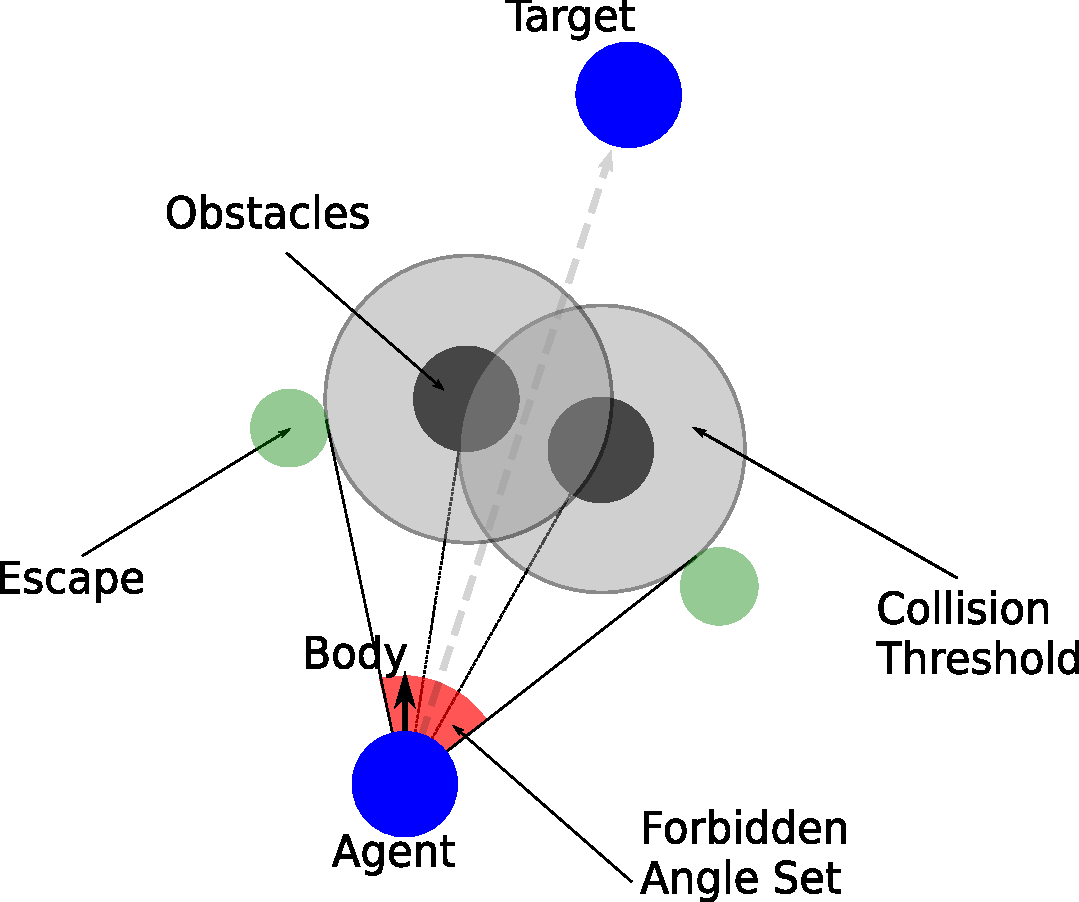
\includegraphics[width=0.3\textwidth]{figures/ObstacleAvoidance.pdf}
\end{figure}


\begin{algorithm}[H]
\caption{Escape Angle Set Calculation}
\begin{algorithmic}[1]
\begin{footnotesize}
\STATE {\bf Input: }$Obstacles = \lbrace O_{1},O_{2},...,O_{n} \rbrace $
\STATE {\bf Output: }$EscapeAngleSet$
\STATE
\FOR{$i = 1 \textbf{ to } n$}
\STATE find $LeftEscapeAngle_i$ for obstacle $O_i$
\STATE find $RightEscapeAngle_i$ for obstacle $O_i$
\ENDFOR
\STATE $EscapeAngleSet = \emptyset$
\FOR{$i = 1 \textbf{ to } n$}
\IF{$LeftEscapeAngle_i \not\in [LeftEscapeAngle_j,RightEscapeAngle_j], \forall  j\neq i$}
\STATE $EscapeAngleSet = EscapeAngleSet \cup \{LeftEscapeAngle_i\}$
\ENDIF
\IF{$RightEscapeAngle_i \not\in [LeftEscapeAngle_j,RightEscapeAngle_j], \forall  j\neq i$}
\STATE $EscapeAngleSet = EscapeAngleSet \cup \{RightEscapeAngle_i\}$
\ENDIF
\ENDFOR
\RETURN $EscapeAngleSet$
\end{footnotesize}
\end{algorithmic}
\end{algorithm}

\end{itemize}

	
	
    \item[Walk to Ball]
	\item[On Ball Action]
    \item[Walk to Coordinate]
    \item[Walk To Direction]
    \item[Walk With Ball To Direction]    
    \end{description}
   
    
  \end{frame}
  
  \subsection*{Communication}
  \frame
  {
    \frametitle{Communication}

   
    
  }
  
  \section{Team Coordination}

  \begin{frame}[allowframebreaks]

    \frametitle{Messages and Communication}
    
    \begin{algorithm}[H]
\caption{Coordination Algorithm}
\label{CoordinationAlgorithm}
\begin{algorithmic}[1]
\begin{footnotesize}
\STATE {\bf Input: }$Coordination Messages = \lbrace M_{1},M_{2},...,M_{N-1} \rbrace, N = number of players $
\STATE {\bf Output: }$Actions = \lbrace A_{1},A_{2},...,A_{N-1} \rbrace$
\IF {$ Step = 1$ }
\STATE $B \leftarrow Update Beliefs() $
\ELSIF {$ Step = 2$ }
\STATE $S \leftarrow Coordination Splitter(B) $
\ELSIF {$ Step = 3$ } 
\STATE $A_{p} \leftarrow Active Positions(B,S) $
\ELSIF {$ Step = 4$ }
\STATE $A_{c} \leftarrow Active Coordination(A_{p},S) $
\ELSIF {$ Step = 5$ }
\STATE $ F \leftarrow TeamFormation(B) $
\STATE $ R \leftarrow Role Assignment(A_{c},B,F) $
\STATE $ S_{p} \leftarrow Support Positions(R,F,S) $
\ELSIF {$ Step = 6$ }
\STATE $ Support Coordination(R,F,S,B,A_{c},S) $
\ENDIF
\end{footnotesize}
\end{algorithmic}
\end{algorithm}
    
  \end{frame}

  \frame
  {
    \frametitle{Coordination�s Beliefs}

   
    
  }
  
  \frame
  {
    \frametitle{Subsets in Coordination}
 
  }
  
  \frame
  {
    \frametitle{Coordination Splitter}
 
  }
  
  \frame
  {
    \frametitle{Soccer Field Value}
 
  }
  
  \frame
  {
    \frametitle{Active Positions}
 
  }
  
  \frame
  {
    \frametitle{Active Coordination}
 
  }
  
  \frame
  {
    \frametitle{Team Formation}
 
  }
  
  \frame
  {
    \frametitle{Role Assignment Function}
 
  }
  
  
  \frame
  {
    \frametitle{Positions for Support Subset}
 
  }
  
  \frame
  {
    \frametitle{Support Coordination}
 
  }
  
  \frame
  {
    \frametitle{Mapping Cost}
 
  }

  \section{Results}

  \frame
  {
    \frametitle{Movement}

  }
  
  \frame
  {
    \frametitle{Communication}

  }


  \frame
  {
    \frametitle{Coordination}

  }

  \frame
  {
    \frametitle{Matches}

  }

  \section{Conclusion}

  \frame
  {
    \frametitle{Future Work}

  }

  \frame
  {
    \frametitle{}

  }


\end{document}
